\documentclass[10pt]{article}

\usepackage{tikz}
\usetikzlibrary{automata, positioning, arrows}
\tikzset{
->,  % makes the edges directed
%>=stealth’, % makes the arrow heads bold
node distance=3cm, % specifies the minimum distance between two nodes. Change if necessary.
every state/.style={thick, fill=gray!10}, % sets the properties for each ’state’ node
initial text=$ $, % sets the text that appears on the start arrow
}


\begin{document}
\begin{figure}[ht] % ’ht’ tells LaTeX to place the figure ’here’ or at the top of the page
\centering % centers the figure
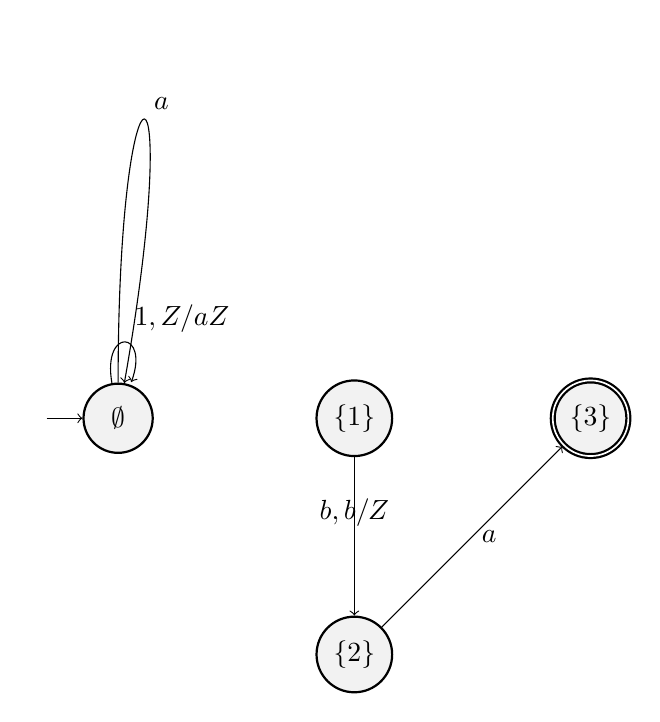
\begin{tikzpicture}
\node[state, initial, initial where=left] (0) {$\emptyset$};
\node[state, right of=0] (1) {$\{1\}$};
\node[state, below of=1] (2) {$\{2\}$};
\node[state, accepting, right of=1] (3) {$\{3\}$};
\path[->] (0) edge [in=70,out=100,loop] node[auto] {$1,Z/aZ$} (0);
\path[->] (0) edge [in=80,out=90,loop,distance=4.5cm] node[auto] {$a$} (0);
\draw 
(1)   edge[above] node{$b,b/Z$} (2)
(2)   edge[right] node{$a$} (3);
\end{tikzpicture}
\end{figure}

\end{document}
